\chapter{Background}
%labels will help you to reference to certain images, tables, chapters, section, and so on...
\label{background}

%DELETEME: This chapter will cover all of your background information and related work. Background and related work are directly related to your thesis. Please do not place irrelevant content here which is a common mistake. Citing will be handled in the appendices.

%DELETEME: Related work respresents results from work that handled the same or a similar problem that you are addressing. This work might have used a different approach or might not have been that successful. Finding a paper / work that solved your problem in the same way you were planning to do is not good and you should contact your supervizor for solving this issue. Again, each paper / work has to be connected to your approach: other papers might have not chosen an optimal solution; they might not have been taking care of essential aspects; they might have chosen a different approach and you believe, yours will work better ...

%###################################################################################
%###################### Related work  ########################################
%###################################################################################

\section{Related Work}
\todo{move / remove what is irrelevant
	\textbf{topology of bots}\\
	\textbf{by platform:}
	-API.ai / 
	Facebook Messenger Chatbots /	
	-wit.ai /
	-motion.ai / Flask
	\\
	\textbf{by category}\\
	- leisure /
	- \href{https://www.forbes.com/sites/tomaslaurinavicius/2017/04/24/facebook-messenger-bots/\#4f61c16a66d8}{fun bots}  / 
	- productivity / 
	- more (graph from voicelabs report) \\
	- what are classic use cases for their use with prominent examples?\\ Booking tickets (e.g. airline bot)\\ %KLM
	- quick survey of respective 'AppStores'\\
	\textbf{by purpose}\\
	-physical locations (home, office, car, phone, in a business)\\
	Information bots\\
	\textcolor{magenta}{
		- mention available service types (information system as a "webpage/database")\\
		- vs an interactive bot that gives you customized information on demand
		hier soll der D115 Anwendungsfall "Beauskunftung" kurz erl\"autert werden\\
	}
	social bots\\
	\textcolor{magenta}{
		- with advantages / disadvantages\\
		- fake news / online reviews\\
	}
	more on AI in bots (optional)\\
	\textcolor{magenta}{
		- use of ML\\
		Handyversicherungsbeispiel\\
		- from business perspective, the bot is aiming to sell more polices,\\ 
		- the bot tries to determine if there is a nuance in the user's answer (machine acting as a judge!)
		- e.g. ``how did the phone fall off``
		- MKTG - Aufwand
		}
	
	
	\textbf{by use case:}\\
	- Wienbot\\
	- Singapore / LA /...\\
	
	
}


Getting started with Alexa platform for the first time might seem a little overwhelming especially since amazon is constantly working on the interface and the sdk 
Throughout the course of this thesis these major changes occurred 

Explain what the ASK SDK does

%Archetype.  Esoterik.   Artifact


%DELETEME: Background represents underlying knowledge that is required to understand your work. The expected knowledge level of your readers can be set to the one of a bachelor or master student who just finished his studies (depending on what kind of thesis you are writing). This means that you do not need to describe how computers work, unless your thesis topic is about this. Everything that an avarage alumni from your field of studies should know does not need to be described. It turn, background information that is very complex and content-wise very near to you problem, can be placed in the main parts. Everyting else should be written here. Note: it is important to connect each presented topic to your thesis. E.g. if you present the ISO/OSI layer model you should also write that this is needed to understand the protocols you plan to develop in the main parts.
%###################################################################################
%###################### State of the Art  ########################################
%###################################################################################
\section{State of the Art}

In this section, we conduct a short survey of problems we can face with natural language

survey of available 
We also di
Natural Language

%IFTTT Applets for voice commands


\todo{ 2 \P \\
	
	\textbf{- Chatbot vs. human: }
	%what we used to do with facets vs a search mask predicting possible facets - we are at a stage where bots are like altavista..u tell alexa to open a skill like u tell altavista to look in pics or go to lexisnexis to do reserach. we are yet to reach the state of watson like google is to searches
	Analyze differences between bot and human response\\
	%human says long sentences and there is a fluid transition between dialog and monologue 
	-disadvantage: a bot wants a sentence broken down in small pieces to avoid errors in lengthy interpretation\\
	% otherwise, error margin too large.\\
	% this has to do with human language complexity.\\
	- \textbf{Why can't robots understand us:} language ambiguities - the need to understand context\\
	--Syntactical: Homonyme\\ %fly, fly,  presently I’ll present you a present - now, give, gift
	--Semantic:  Methaphors, %“it’s raining cats and dogs”
	sarcasm, %“oh yea, sounds very exciting”
	and puns\\
	--dialects: enunciations\\
	--underlying grammar\\ %“what makes you abcd just now, ELIZA
	--underlying sentiment\\
	-\textbf{NLP Progress:} How does it help in enriching the bot experience\\
	--neural networks: help understanding language patterns and get better over time\\
	--thought vectors: helps connect different words with related meaingns\\
	- \textbf{wrap-up:} can bots replace serivces offered by humans?
	-- mention transition from facets (Altavista) to metasearches to all-in-one (Google). \\
	-- chatbots as enablers in customer service industry\\
	-- conclusion: Although not impossible, it is a bit too far-fetched at this stage.\\
}




\subsection{Amazon Web Services and the Alexa Platform}

Alexa is the cloud-based voice Service by Amazon powering millions of devices \inote{number of requests, ...} including its own-branded devices like Echo, Echo Dot, Tap, FireTV as well as cross-platform on Apple's iPhone
\todo{	
	-  Alexa Skills Kit+ Amazon Voice Services\\
	- mention how ability to react to everything is centralized at alexa somewhere \textbf{talk about SKILLS}\\
	- ability to retain sessions (explain requests/responses - GET/POST)\\
	- fullfilling intents\\
	- nested handlers\\
		\\
		skill service: code - business logic - handles json requests
		skil interface: configuration (developer portal)
		\\
	- difference to Lex \& Polly\\
	\href{https://stackoverflow.com/questions/42982159/differences-between-using-lex-and-alexa}{diff alexa lex}
		
	- Major prob: lex is not in german
- \href{https://www.youtube.com/watch?v=QxgdPI1B7rg}{Alexa Documentation}
}
\subsection{Amazon Voice Service}
just like other common chat bot constructs, Alexa Skills Kit (ASK) divides the building model into intents~\ref{intents}, utterances and slots. The Fulfillment part is taken care of through Amazon Lambda contains the programming \inote{and business} logic to the interface
\begin{itemize}
	\item Intents
	\
\end{itemize}

\subsection{Node.js}

AWS Lambda supports multiple runtime environments including Python, Java, C\# and Go. However, we use Node.js due to its event-driven nature and to take advantage of its non-blocking I/O model. Being single-threaded, Node.js guarantees high performance at large scale with large volumes of requests considered. With its JavaScript (ECMAScript) foundation, it is becoming a standard in web-apps. 
\todo{
	- Server-side, browser side (Chrome V8), App layer, data layer\\
	- because it can read our JSON easily and fast
	- talk about Methodenaufbau (syntax) and firing events
}

\subsection{Alexa Interfaces}
- Echosim.io
- Devices
- Reverb (iOS)

%###################################################################################
%###################### Topic A             ########################################
%###################################################################################
\section{D115}
\textcolor{magenta}{
	- summarize infobroschuere\_ BMI08324\_screen\_barrierefrei.pdf\\
	-Use case im Detail\\
	-Welche Daten gibt es?\\	  
	-Was sind die Erwartungen?\\ 	
	- wie kann man die G\"ute des Systems beurteilen?\\   
	- Meist sollte man in diesem Kapitel die L\"osung schon im Auge haben, um die Erwartungen so zu formulieren, dass die L\"osung auch geeignet ist?\\ 
}


%###################################################################################
%###################### Topic B             ########################################
%###################################################################################
\section{Frameworks and Data Structures \textcolor{magenta}{(change title)}}

\textcolor{magenta}{-AL: Ich w\"urde erst etwas die Algorithmen und Datenstrukturen (Textanalyse, JSON, ggf. Graphen beschreiben. 
	-AL: Anschlie{\ss}end die Frameworks vorstellen\\ 
	-AL: Wichtig ist: Aus den Beschreibungen eine Schlussfolgerung ableiten, welche Art von L\"osung entwickelt werden soll.\\
for current bot: \\
- Lucene \textbf{as the golden standard}: spell check, unscharfe suche, Tika / detect language / ... \\
- Solr
- explain what's an intent, whats a slot
\url{https://service.berlin.de/virtueller-assistent/virtueller-assistent-606279.php}
\url{https://www.itdz-berlin.de/}
}


\subsection{Intents and Slots} \todo{explain json}

OnLaunch
IntentHandler
intent is triggered by utterence
account verlinkungen etc

%\Tree [.Dienstleistungen.json created [.VP [.V is ] NP ] ]
%
%\Tree[.Dienstleistungen.json 	
%	[.NP [.Det \textit{the} ]
%		[.N\1 [.N \textit{package} ]]]
%	[.I\1 [.I \textsc{3sg.Pres} ]
%		[.VP [.V\1 [.V \textit{is} ]
%			 	   [.AP [.Deg \textit{really} ]
%				  		[.A\1 [.A \textit{simple} ]
%							  \qroof{\textit{to use}}.CP ]]]]]]]

provided in JSON for value lookup, there are

\begin{figure}[h!]
	\caption{\lstinline|Dienstleistungen.json|  - Primary Nodes}
	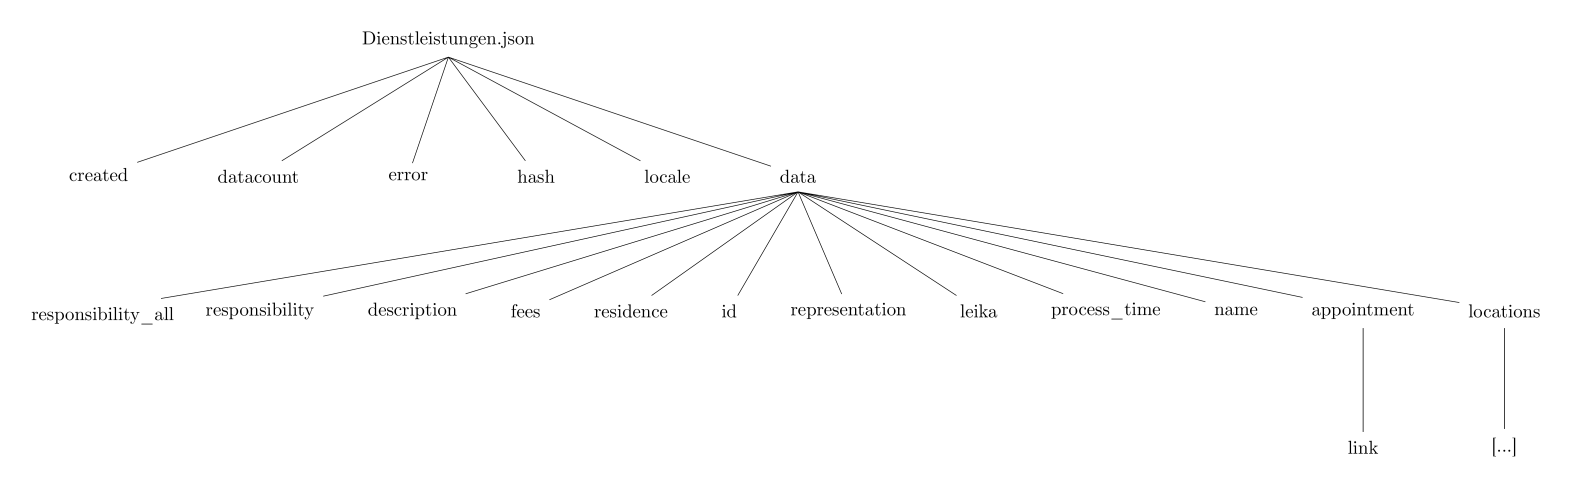
\includegraphics[width=\textwidth]{DLprim}
\end{figure}

\begin{figure}[h]
	\caption{\lstinline|Dienstleistungen.json| - secondary Nodes}
	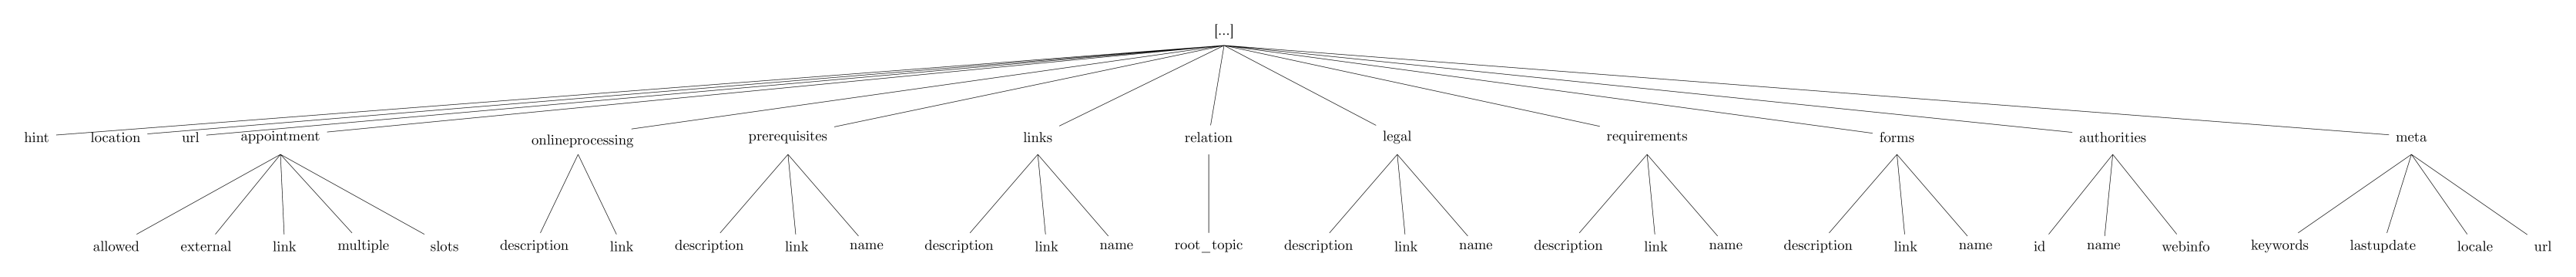
\includegraphics[width=\textwidth]{DLsec}
\end{figure}

\begin{itemize}
	\item 616 Intents as \lstinline|data|, each containing
	\todo{missing variables e.g. are required papers, flag: persönliche Vorsprache ja nein, ...}
	\begin{itemize}
		\item \lstinline|<string> responsibility| denoting in which city halls a service is available
		\item \lstinline|<boolean> responsibility_all| a flag set to true in case the service is available in all local authority offices / service points
		\item \lstinline|<HTML list string> description| not unified and includes text
		\item  \lstinline|<string> not unified and might need to have an \lstinline|int| added to it and set to 0 in case service is free
		\item \lstinline|<int>residence|
		\item \lstinline|<int>id|
		\item \lstinline|representation|
		\item \lstinline|<long>leika|
		\item \lstinline|<string> process_time| need to derive minimum, average and maximum service times instead of a string, as well as conditions 
		\item \lstinline|<string> name| the name of the service that would make sense to a human
		\item \lstinline|<node> appointment| with 
		\begin{itemize}
			\item \lstinline|link| (Key value with URL to /terminveinbarung page) - check if orphan or if it is for each beh\"orde and in that case how it gets the right one
		\end{itemize}	 
		\item \lstinline|<node> locations| 
		\begin{itemize}
			\item \lstinline|hint|
			\item \lstinline|<int> location| one of the 12 authorities
			\item \lstinline|url| of that service at that authority
			\item \lstinline|<node> appointment| (a second one)
			\begin{itemize}
				\item 
			\end{itemize}
		\end{itemize}
		
		\item \lstinline|<node> onlineprocessing|
		\item \lstinline|<node> prerequisites|
		\item \lstinline|<node> links|
		\item \lstinline|<node> relation|
		\item \lstinline|<node> legal|
		\item \lstinline|<node> requirements|
		\item \lstinline|<node> forms|
		\item \lstinline|<node> authorities|
		\item \lstinline|<node> meta|										
	\end{itemize}
\end{itemize}

\section{currently deployed bot}


\textcolor{magenta}{
- dienstleistungen.json structure (finding the info through hierarchical nodes)\\
- interpreting the nodes as intents
- traversing the nodes (one level up then to next node)
- no session/no persistence
%x	x	x
%ooo ooo ooo
%try first, go to second (kosten, zeit, rechtsgrundlage, ..) skip one if it has already been suggested.. hinweis..that is built into the xml
%
%the live service is different than the one at DAI
}

%###################################################################################
%###################### Topic C             ########################################
%###################################################################################
\section{Implementation Possibilities}

\textcolor{magenta}{
- structure of Hitlist on berlin.de  is provided by ITDZ -  as opposed to Versicherungsfirma z.B (ML tries to detect irregular patterns in case customer is lying).
- unfortunately forums vs. FAQs did not work. if i want assistance, i want the customer to tell me the model number - and forums have mostly Schrott!\\
what the bot curently achieved is at least not give wrong answers, sometimes says idk but it doesnt confuse u. same attitude like in german shops (nur unpassende antworten sind frustrierend!\\
\\
-Vorgehensweise: XML -> index \"uber Lucene - >solr knoten...based on sth like when i say \" am 10. august\" it gets me masalan events..aha august ist ein monat, monat relates to calendar, calendar relates to events
}